\documentclass[a4paper,journal]{IEEEtran}
%\documentclass[conference]{IEEEtran}
%for using the therefore symbol
%\usepackage{amssymb}
%end

\usepackage[utf8]{inputenc}
\usepackage{graphicx}
\usepackage{float}
\usepackage{color, colortbl}
\usepackage{xcolor}
\usepackage{array}
\usepackage{multirow}
\usepackage{footnote}
\usepackage{cite}
%The below is used to add notes to tables without disrupting the IEEEtran format
\usepackage{threeparttable}
%Multiple figures in a row
%\usepackage{caption}
%\usepackage{subcaption}
\usepackage{amsmath}
\usepackage{mathtools}
%Algorithms
\usepackage[linesnumbered,vlined]{algorithm2e}

\usepackage[hyphens]{url}

% Disable below if wanting to comply exclusively to conference mode of IEEEtran
% \IEEEoverridecommandlockouts


\usepackage{lipsum}

\begin{document}
%opening
 \title{Building The Next MAC for WLANs}


%A more simple output, useful when involving people from different affiliations
  %\author{
    %  \IEEEauthorblockN{Luis Sanabria-Russo\IEEEauthorrefmark{0}, Jaume Barcelo\IEEEauthorrefmark{0}, Boris Bellalta\IEEEauthorrefmark{0}}\\
      %\IEEEauthorblockA{\IEEEauthorrefmark{0}Universitat Pompeu Fabra, Barcelona, Spain
      %\\\{luis.sanabria, jaume.barcelo, boris.bellalta\}@upf.edu}
  %}

\author{Luis Sanabria-Russo \\
		NeTS Research Group at\\
		Universitat Pompeu Fabra, Barcelona, Spain\\
		\texttt{Luis.Sanabria@upf.edu}}

%This is the style of three columns, as indicated in IEEEtran
% \author{\IEEEauthorblockN{Luis Sanabria-Russo}
%  \IEEEauthorblockA{Department of Information\\
%  and Communications Technologies\\
%  Universitat Pompeu Fabra\\
%  Barcelona, Spain\\
%  Email: luis.sanabria@upf.edu}
%  \and
%  \IEEEauthorblockN{Jaume Barcelo}
%  \IEEEauthorblockA{Department of Information\\
%  and Communications Technologies\\
%  Universitat Pompeu Fabra\\
%  Barcelona, Spain\\
%  Email: cristina.cano@upf.edu} 
%  \and
%  \IEEEauthorblockN{Boris Bellalta}
%  \IEEEauthorblockA{Department of Information\\
%  and Communications Technologies\\
%  Universitat Pompeu Fabra\\
%  Barcelona, Spain\\
%  Email: boris.bellalta@upf.edu}}


\maketitle

\begin{abstract}

\boldmath Collisions are a main cause of throughput degradation in WLANs. The current contention mechanism used in IEEE 802.11 networks is called Carrier Sense Multiple Access with Collision Avoidance (CSMA/CA). It uses a Binary Exponential Backoff (BEB) technique to randomize each contender attempt of transmitting, effectively reducing the collision probability. Nevertheless, CSMA/CA relies on a random backoff that while effective and totally distributed, in principle is unable to completely eliminate collisions; degrading the network throughput as more contenders attempt to share the channel. Carrier Sense Multiple Access with Enhanced Collision Avoidance (CSMA/ECA) is able to create a collision-free schedule in a totally distributed manner by means of picking a deterministic backoff after successful transmissions. Further, by applying simple extensions to the backoff mechanism of CSMA/ECA it is able to support many contenders in a collision-free schedule, surpassing the achieved throughput of CSMA/CA and providing short-term throughput fairness among contenders.

This work describes CSMA/ECA, its mechanisms to achieve a collision-free schedule with many contenders as well as its performance when coexisting with CSMA/CA nodes. Further, the effects of imperfect clocks over CSMA/ECA's deterministic backoff mechanism and its consequences when attempting to implement the protocol in real hardware are also analysed. %Results are derived from computer simulations using a modified version of an event-based network simulator.

%This work describes CSMA/ECA and its mechanisms to achieve a collision-free schedule with many contenders by providing insightful simulation under different network traffic conditions and hardware anomalies such as an imperfect clock.

\end{abstract}

\begin{IEEEkeywords}
CSMA/ECA, WLAN, MAC, Collision-free, Clock Drift.
\end{IEEEkeywords}

\section{Introduction}\label{introduction}
Wireless Local Area Networks (WLANs or IEEE 802.11 networks~\cite{802Standards}) are a popular solution for wireless connectivity, whether in public places, work environments or at home. This technology works over an unlicensed spectrum in the Industrial, Scientific and Medical (ISM) radio bands (at around $2.4$ or $5$~GHz), offering a good tradeoff between performance and costs; which is a main reason for its popularity. 

The Medium Access Control (MAC) scheme used in WLANs is called Distributed Coordination Function (DCF) and is based on Carrier Sense Multiple Access with Collision Avoidance (CSMA/CA) protocol. It has been widely adopted by manufacturers and consumers, making it very cheap to implement and an ubiquitous technology\footnote{DCF and CSMA/CA will be used interchangeably throughout this work}. Nevertheless, the ever-growing throughput demands from upper layers have proven to be limited by WLANs' MAC~\cite{perahia2008ieee}, which by its nature is prone to collisions that degrade the overall performance as more nodes join the network.

The research community has pushed forward many alternatives to the current MAC in WLANs~\cite{bharghavan1994map,wang2004ncr,cali2000dti,lopez-toledo2006aoi,
barcelo2008lba,bellalta2009vtc,HE,CSMA_ECA,L_MAC2,hui2011epp,barcelo2011tcf}, but when a proposal deviates too much from CSMA/CA or time-critical operations are modified, its hardware implementation as part of WLANs' MAC often becomes unlikely~\cite{WMP}; the standardization process taking many years without certainty of approval~\cite{perahia2008ieee}. 

%Backwards compatibility is paramount, mostly because the existing user base is very big. Also, a suitable candidate to replace CSMA/CA should increase the number of supported contenders while augmenting the offered throughput.

A CSMA/CA replacement should be able to provide advantages in terms of throughput, spectrum efficiency and handle many contenders without sacrificing short-term throughput fairness. Furthermore, to support the existing user base and ease its implementation on real hardware, the new MAC protocol should be backwards compatible.

%Furthermore, due to the proliferation of evermore WiFi-capable devices, it is thought that a suitable replacement should 

A suitable candidate, and the one to be evaluated in this work, is called Carrier Sense Multiple Access with Enhanced Collision Avoidance (CSMA/ECA)~\cite{barcelo2008lba}. It is capable of attaining higher throughput than CSMA/CA by making a modification to the contention mechanism. In CSMA/ECA, nodes pick a deterministic backoff after successful transmissions; constructing a collision-free schedule among successful contenders. This backoff mechanism ensures that more channel time is spent on successfull transmissions rather than recovering from collisions, thus increasing the throughput of the network. Further enhancements, like \emph{Hysteresis} and \emph{Fair Share}~\cite{research2standards} allowed CSMA/ECA to support many more contenders in a collision-free schedule without compromising short-term fairness.

Although many studies have been made analysing the performance of CSMA/ECA~\cite{barcelo2008lba,research2standards,bellalta2009vtc,E2CA_performance}, neither assesses the protocol's backwards compatibility property under different traffic conditions. Furthermore, the impact of imperfect clocks over the deterministic backoff mechanism is also lacking.

%Furthermore, all the aforementioned studies are based on simulation results, bypassing the influence of realistic testing scenarios over the overall network performance.

This work serves as an extension to~\cite{research2standards}, and provides the first simulation results on achieved throughput and suffered delay of CSMA/ECA under different traffic conditions. Further, a short overview of a real hardware implementation of CSMA/ECA alongside future challenges is provided prior the conclusions.

%Further, for the first time it is discussed how different WLANs features would work under CSMA/ECA. These features include: Enhanced Distributed Channel Access' (EDCA) Access Categories (AC) as Quality of Service (QoS), more than one spatial stream with Multiple User Multiple-input Multiple-output (MU-MIMO) and the implementation of CSMA/ECA in ad-hoc networks.

%Results are derived from computer simulations over a customised version of the COST~\cite{COST} event-based simulator.

The rest of this work is divided as follows: an overview of similar distributed and collision-free MAC protocols for WLANs is provided in  Section~\ref{relatedWork}. CSMA/ECA, as well as its properties for allocating many contenders in a collision-free schedule are explained in Section~\ref{introProtocol}. Section~\ref{simulations} details the simulation environment for testing CSMA/ECA, while Section~\ref{results} explains the results. An overview a CSMA/ECA real-hardware implementation is compiled in Section~\ref{EDCA}, followed by conclusions in Section~\ref{conclusions}.

%goes through the prototyping of CSMA/ECA in real hardware. The results for the simulation and prototypes are presented in Section~\ref{prototypeResults}. Conclusions are drawn in Section~\ref{conclusions}.


%{\color{blue}\lipsum}

\section{Related Work}\label{relatedWork}
Time in WLANs is divided into tiny empty slots of fixed length $\sigma_{e}$, collisions and successful slots of length $\sigma_{c}$ and $\sigma_{s}$, respectively. Collision and successful slots contain collisions or successful transmissions, making them several orders of magnitude larger than empty slots ($\sigma_{e}\ll\min(\sigma_{s},\sigma_{c}))$. One of the effects of collisions is the degradation of the network performance by wasting channel time on collisions slots. 

Big advances in the WLANs PHY~\cite{perahia2008ieee,6191306} push the community towards the development of MAC protocols able to take advantage of a much faster PHY. By reducing the time spent in collisions nodes are able to transmit more often, which in turn translates to an increase in the network throughput. Further, the upcoming MAC protocols for WLANs should work without message exchange between contenders, that is, work in a totally distributed fashion in order to avoid injecting extra control traffic that may reduce the data throughput.

The followings are MAC protocols suitable for replacing the current standard in WLANs, distributed and capable of attaining greater throughput than CSMA/CA by constructing a collision-free schedule.

\subsection{Zero Collision MAC} 

Zero Collision MAC (ZC-MAC)~\cite{ZMAC} achieves a zero collision schedule for WLANs in a totally distributed way. It does so by allowing contenders to reserve one empty slot from a  predefined virtual schedule of $N$-slots in length. Backlogged stations pick a slot in the virtual cycle to attempt transmission. If two or more stations pick the same slot in the cycle, their transmissions will eventually collide; forcing the involved contenders to randomly and uniformly select other empty slot from those detected empty in the previous cycle plus the slot where they collided. When all $M$ stations reserve a different slot, a collision-free schedule is achieved.

ZC-MAC is able to outperform CSMA/CA under different scenarios. Nevertheless, given that the length of ZC MAC's virtual cycle has to be predefined without actual knowledge of the real number of contenders in the deployment, the protocol is unable to provide a collision-free schedule when $M>N$. Furthermore, if $N$ is overestimated ($N\gg M$), the fixed-width empty slots between each contender's successful transmission are no longer negligible and contribute to the degradation of the network performance.

\subsection{Learning-MAC}

Learning-MAC~\cite{L_MAC} is another MAC protocol able to build a collision-free schedule for many contenders. It does so defining a \emph{learning strength} parameter, $\beta\in(0,1)$. Each contender starts by picking a slot for transmission $s$ of the schedule $n$ of length $C$ at random with uniform probability. After a contender picks slot $s(n)$, its selection in the next schedule, $s(n+1)$, will be conditioned by the result of the current attempt. (\ref{success}) and (\ref{collision}) extracted from~\cite{L_MAC} show the probability of selecting the same slot $s(n)$ in cycle $n+1$.

\begin{equation} \label{success}
		\left. \begin{aligned}
			p_{s(n)}(n+1)&=1,\\
			p_{j}(n+1)&=0,
		\end{aligned}
	\right\}
	\qquad \text{\emph{Success}}
\end{equation}
\begin{equation} \label{collision}
	\left. \begin{aligned}
			p_{s(n)}(n+1)&=\beta p_{s(n)}(n),\\
			p_{j}(n+1)&=\beta p_{j}(n)+\frac{1-\beta}{C -1},
		\end{aligned}
	\right\}
	\qquad \text{\emph{Collision}}
\end{equation}
\\
for all $j\neq s(n),~j\in \{1,\dots ,C\}$. That is, if a station successfully transmitted in $s(n)$, it will pick the same slot on the next schedule with probability one. Otherwise, it follows~(\ref{collision}).

The selection of $\beta$ implies a compromise between fairness and convergence speed, which the authors determined $\beta=0.95$ to provide satisfactory results.

L-MAC is able to achieve higher throughput than the current MAC with a very fast convergence speed. Nevertheless, the choice of $\beta$ suppose a previous knowledge of the number of empty slots ($C-N$, where $N$ is the number of contenders), which is not easily available to the current MAC or may require a centralised entity~\cite{barcelo2011tcf}.

Further extensions to L-MAC introduced an \emph{Adaptative} schedule length in order to increase the number of supported contenders in a collision-free schedule. This adaptive schedule length is doubled or halved depending on the presence of collisions or many empty slots per schedule, respectively. The effects of reducing the schedule length may provoke a re-convergence phase which can result in short-term fairness issues. 
%Furthermore, L-MAC is unable to achieve a collision-free schedule unless $N\leq C$.

\section{Carrier Sense Multiple Access with Enhanced Collision Avoidance (CSMA/ECA)}\label{introProtocol}
CSMA/ECA~\cite{barcelo2008lba} is a totally distributed and collision-free MAC for WLANs. It differs from DCF in that it picks a deterministic backoff, $B_{d}=CW_{\min}/2$ after successful transmissions; where $CW_{\min}$ is the minimum contention window of typical value $CW_{\min}=16$. By doing so, contenders that successfully transmitted on schedule $n$, will transmit without colliding with other successful nodes in future cycles.

Collisions are handled as in DCF, which is described in Algorithm~\ref{alg:CSMA_CA}. In Algorithm~\ref{alg:CSMA_CA}, the node starts by setting the retransmissions counter and backoff stage to zero ($r\in[0,R]$ and $k\in[0,m]$ respectively; $m$ is the maximum backoff stage of typical value $m=5$, and $R$ is the retransmissions limit with typical value $R=m+1$), then generates a random backoff, $B$. When the Acknowledgement (\emph{ack}) for a sent packet is not received by the sender a collision is assumed. Upon collision, the involved nodes will double their contention window by incrementing their backoff stage in one and picking a random backoff, $B\in[0,2^{k}CW_{\min}]$. This procedure is described between Line~\ref{collision} and~\ref{finalCollision} of Algorithm~\ref{alg:CSMA_CA}.

Algorithm~\ref{alg:CSMA_ECA} provides an explanation of CSMA/ECA deterministic backoff mechanism, which main difference with CSMA/CA (and therefore with Algorithm~\ref{alg:CSMA_CA}) relies on the selection of a deterministic backoff after a successful transmission (compare Line~\ref{randomBackoff} in Algorithm~\ref{alg:CSMA_CA} with Line~\ref{deterministicBackoff} in Algorithm~\ref{alg:CSMA_ECA}). Figure~\ref{fig:BECA-example} shows an example of CSMA/ECA dynamics with four contenders.

\begin{algorithm}[ht!!!]
\While{the device is on}
{
  %\tcc{Initialize retransmission attempts.}
  $r \leftarrow 0$; $k \leftarrow 0$\;
  %\tcc{Initialize backoff counter.}
  $B \leftarrow \mathcal{U}[0,2^k{\rm{CW}_{min}}-1]$\;
  \While{there is a packet to transmit}{
    %\tcc{Initialize $a$.}
    \Repeat{($r = R$) or (success)}{
      %\tcc{First, backoff.}
      \While{$B>0$}{
        wait 1 slot\;
        $B \leftarrow B-1$\;
      }
      \colorbox{yellow}{Attempt transmission of 1 packet;}\\
      \If{collision}{\label{collision}
        %\tcc{Random backoff.}
        $r \leftarrow r+1$\;
        $k \leftarrow \min (k+1,m)$\;
        $B \leftarrow \mathcal{U}[0, 2^k {\rm{CW}_{min}} -1]$\;\label{finalCollision}
      }
    }
    $r \leftarrow 0$\;
    \colorbox{yellow}{$k \leftarrow 0$;}\\
	 \eIf{success}{
      %\tcc{Random backoff.}
      \colorbox{yellow}{$B \leftarrow \mathcal{U}[0,2^{k}{\rm{CW}_{min}}-1]$;}\\\label{randomBackoff}
    }
    {
      Discard packet\;
      $B \leftarrow \mathcal{U}[0,2^k {\rm{CW}_{min}}-1]$\;
    }
  }
  Wait until there is a packet to transmit\;
}
\caption{\small{CSMA/CA. $r$ indicates the number of retransmission attempts, while $R$ is the maximum retransmission attempts limit; when it is reached, the packet waiting for transmission is dropped.}}
\label{alg:CSMA_CA}
\end{algorithm}

\begin{algorithm}[ht!!!]
\While{the device is on}
{
  $r \leftarrow 0$ ; $k \leftarrow 0$\;
  $B \leftarrow \mathcal{U}[0,2^k{\rm{CW}_{min}}-1]$\;
  \While{there is a packet to transmit}{
    %\tcc{Initialize $a$.}
    \Repeat{($r = R$) or (success)}{
      %\tcc{First, backoff.}
      \While{$B>0$}{
        wait 1 slot\;
        $B \leftarrow B-1$\;
      }
      \colorbox{yellow}{Attempt transmission of 1 packet;}\\
      \If{collision}
      {
        %\tcc{Random backoff.}
        $r \leftarrow r+1$\;
        $k \leftarrow \min (k+1,m)$\;
        $B \leftarrow \mathcal{U}[0, 2^k {\rm{CW}_{min}} -1]$\;
      }
    }
    $r \leftarrow 0$\;
    \colorbox{yellow}{$k \leftarrow 0$;}\\
    \eIf{success}{
      %\tcc{Random backoff.}
      \colorbox{yellow}{$B_{d} \leftarrow (2^{k}{\rm{CW}_{min}})/2-1$\;}\label{deterministicBackoff}\\
	 $B \leftarrow B_{d}$\;
    }
    {
      Discard packet\;
      $B \leftarrow \mathcal{U}[0, 2^k {\rm{CW}_{min}}-1]$\;
    }
  }
  Wait until there is a packet to transmit\;
}
\caption{\small{CSMA/ECA.}}
\label{alg:CSMA_ECA}
\end{algorithm}

%where $k$ is reset ($k=0$) after each successful transmission and $m$ is the maximum backoff stage of typical value $m=5$

\begin{figure*}[tb]
\centering
  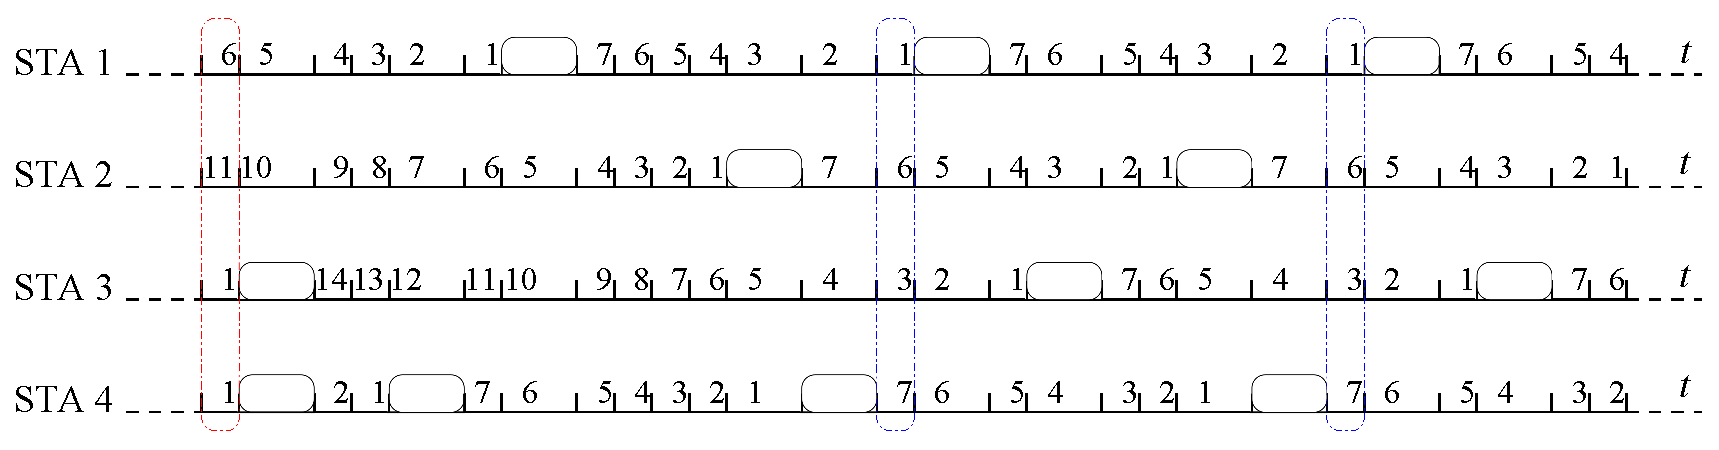
\includegraphics[width=0.8\linewidth]{figures/basicECA.eps}
  \caption{CSMA/ECA example in saturation}
  \label{fig:BECA-example}
\end{figure*}

In Figure~\ref{fig:BECA-example}, the \emph{STA-\#} labels represent stations willing to transmit. The horizontal lines represent a time axis with each number indicating the amount of empty slots left for the backoff to expire. Stations willing to transmit begin the contention for the channel by picking a random backoff, $B$. The first outline highlights the fact that stations STA-3 and STA-4 will eventually collide because they have selected the same $B$. After recomputing the random backoff, STA-4's attempt results in a successful transmission, which instructs the node to pick a deterministic backoff, $B_{d}=7$ in this case. By doing so, all successful STAs will not collide among each other in future cycles.

Collision slots being orders of magnitude larger than empty slots degrade the network performance. When CSMA/ECA builds the collision-free schedule all contenders are able to successfully transmit more often, increasing the aggregated throughput beyond DCF's. Figure~\ref{fig:BECA} shows the achieved throughput of CSMA/ECA and CSMA/CA, alongside the Jain's Fairness Index (JFI)~\cite{JFI}.

\begin{figure}[tb]
\centering
  \includegraphics[width=0.7\linewidth, angle=-90]{figures/DCF-vs-ECA.eps}
  \caption{CSMA/ECA example in saturation}
  \label{fig:BECA}
\end{figure}

Referring to Figure~\ref{fig:BECA}, CSMA/ECA is able to achieve an aggregated throughput that goes beyond CSMA/CA up until the number of contenders ($N$) is greater than $B_{d}=7$. Beyond this point, the network will have a mixed behavior relating to backoff mechanisms: some nodes will successfully transmit and pick a deterministic backoff while others will collide due to the lack of empty slots and return to a random backoff. As more contenders join the network, CSMA/ECA performance will approximate to CSMA/CA's.

The \emph{JFI for CSMA/ECA} and \emph{JFI for CSMA/CA} curves in Figure~\ref{fig:BECA} show the Jain's Fairness index for both protocols. Both protocols have a JFI equal to one, which suggests that the available throughput is shared evenly among all stations.

	\subsection{Supporting many more contenders}\label{moreContenders}
	As was mentioned before, CSMA/ECA is only able to build a collision-free schedule if the number of contenders $N$, is less or equal than $B_{d}$. When $N > B_{d}$, collisions reappear. 
	
	To be able to attain a collision-free schedule even when the number of contenders exceeds $B_{d}$, we introduce \emph{Hysteresis}. Hysteresis is a property of the protocol that instructs nodes not to reset their backoff stage ($k$) after successful transmissions, but to pick a deterministic backoff $B_{d}=CW(k)/2$; where $CW(k)=2^{k}CW_{\min}$. This measure allows the adaptation of the schedule length, admitting many more contenders in a collision-free schedule.
	
	Hysteresis enables CSMA/ECA nodes to have different schedules ($B_{d}$), carrying the undesired effect of unevenly divide the channel time among contenders (i.e., some nodes will have to wait more in order to attempt transmissions).
	
	This unfairness issue is solved by instructing nodes at backoff stage $k$ to transmit $2^{k}$ packets on each attempt, thus proportionally compensating those nodes at higher backoff stages. This additional extension to CSMA/ECA is called \emph{Fair Share}. CSMA/ECA with Hysteresis and Fair Share will be referred to as CSMA/ECA$_{\text{Hys+FS}}$ in order to distinguish it from what was described until this point.
	
	The idea of allowing the transmission of more packets to stations that transmit less often was initially proposed by Fang et al. in~\cite{L_MAC}. It was later adapted to CSMA/ECA$_{\text{Hys}}$ and named Fair Share in~\cite{research2standards}. Figure~\ref{fig:fairness} shows the JFI for CSMA/CA as well as for CSMA/ECA$_{\text{Hys+FS}}$.
	
	\begin{figure}[tb]
	\centering
		\includegraphics[width=0.7\linewidth, angle=-90]{figures/fairness-combined.eps}
		\caption{Fairness comparison with nodes under saturation}
		\label{fig:fairness}
	\end{figure}
	
	In Figure~\ref{fig:fairness}, the only curve deviating from JFI = 1 is \emph{CSMA/ECA with Hysteresis}; suggesting an uneven partition of the channel access time among contenders (which is fixed with Fair Share).
	
	\begin{figure*}[tb]
	\centering
		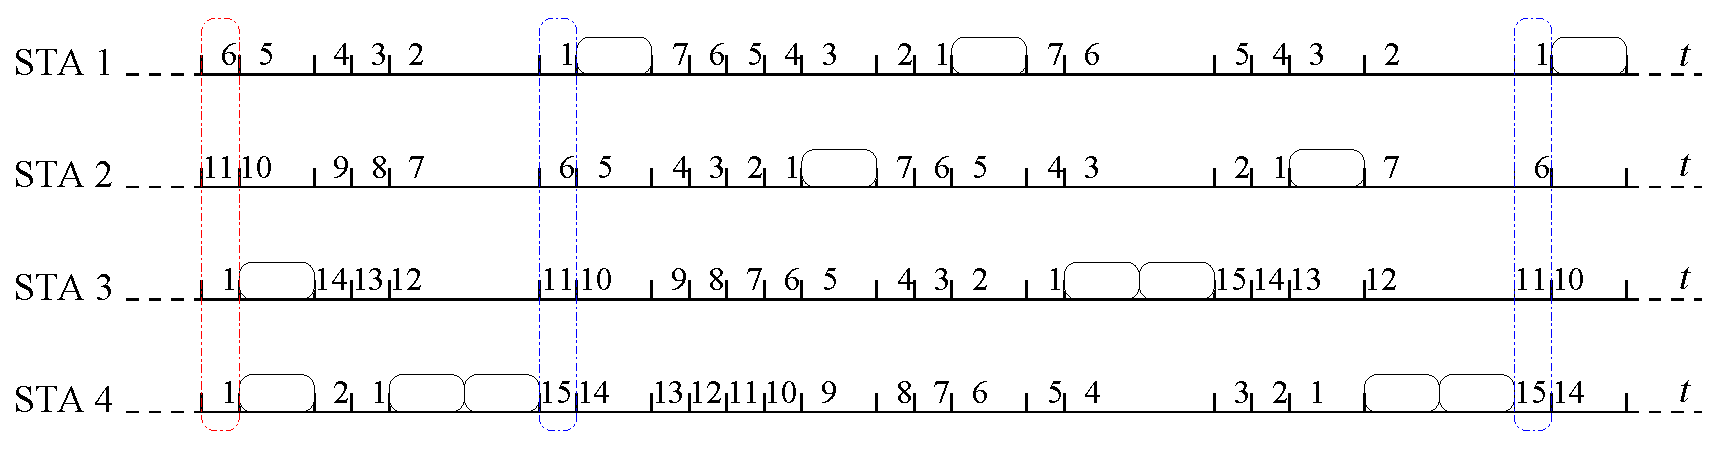
\includegraphics[width=0.8\linewidth]{figures/csma_eca_different_backoff_short.eps}
		\caption{CSMA/ECA$_{\text{Hys+FS}}$ example in saturation ($CW_{\min}=16$)}
		\label{fig:ECA+Hyst}
	\end{figure*}
	
	Algorithm~\ref{alg:fullECA} shows an implementation of CSMA/ECA$_{\text{Hys+FS}}$, while an example of CSMA/ECA$_{\text{Hys+FS}}$ with four contenders is shown in  Figure~\ref{fig:ECA+Hyst}. In the figure the first outline indicates a collision between STA-3 and STA-4, which will provoke an increment on both station's backoff stage ($k'=k+1$). Once STA-4's random backoff expires, CSMA/ECA$_{\text{Hys+FS}}$ instructs the station to transmit $2^{k'}$ packets, and then pick a deterministic backoff, $B_{d}=CW(k')/2$. The same behavior is followed by STA 3.
	
	With Hysteresis and Fair Share, CSMA/ECA$_{\text{Hys+FS}}$ is able to achieve greater throughput than CSMA/CA and for many more contenders, as shown in Figure~\ref{fig:ECA+H+F-throughput} extracted from~\cite{research2standards}. In the figure, the \emph{CSMA/ECA with Hysteresis and Fair Share} curve shows a greater throughput because collisions are eliminated and Fair Share allows nodes to send $2^{k}$ packets upon each transmission.

	\begin{algorithm}[tb]
	\While{the device is on}
	{
	  $r \leftarrow 0$ ; $k \leftarrow 0$\;
	  $b \leftarrow \mathcal{U}[0,2^k\rm{CW}_{min}-1]$\;
	  \While{there is a packet to transmit}{
	    %\tcc{Initialize $a$.}
	    \Repeat{($r = R$) or (success)}{
	      %\tcc{First, backoff.}
	      \While{$B>0$}{
	        wait 1 slot\;
	        $B \leftarrow B-1$\;
	      }
	      \colorbox{yellow}{Attempt transmission of $2^k$ packets;}\\
	      \If{collision}{
	        %\tcc{Random backoff.}
	        $r \leftarrow r+1$\;
	        $k \leftarrow \min (k+1,m)$\;
	        $B \leftarrow \mathcal{U}[0, 2^k  \rm{CW}_{min} -1]$\;
	      }
	    }
	    $r \leftarrow 0$\;
	    %$s \leftarrow 0$\;
	    \eIf{success}{
	      %\tcc{Random backoff.}
	      \colorbox{yellow}{$B_{d} \leftarrow (2^{k}\rm{CW}_{min})/2-1$;}\\
		$B \leftarrow B_{d}$;\\
	    }
	    {
	      Discard packet\;
	      $B \leftarrow \mathcal{U}[0, 2^k \rm{CW}_{min}-1]$\;
	    }
	  }
	  Wait until there is a packet to transmit\;
	}
	\vspace{0.2cm}
	\caption{CSMA/ECA$_{\text{Hys+FS}}$}
	\label{alg:fullECA}
	\end{algorithm}

	\begin{figure}[tb]
	\centering
		\includegraphics[width=0.7\linewidth,angle=-90]{figures/throughput-combined-2.eps}
		\caption{Throughput comparison~\cite{research2standards}}
		\label{fig:ECA+H+F-throughput}
	\end{figure}


	\subsection{CSMA/ECA$_{\text{Hys+FS}}$ vs. Maximum aggregation in CSMA/CA}
	Fair Share is an aggregation mechanism that coupled with the collision-free schedule built by CSMA/ECA$_{\text{Hys}}$ is able to provide greater throughput than CSMA/CA. Figure~\ref{fig:ECA-vs-DCF-maxAgg} shows the achieved aggregated throughput for CSMA/ECA$_{\text{Hys+FS}}$ and CSMA/CA with nodes sending $2^m$ packets in each attempt. This CSMA/CA behavior will be called CSMA/CA$_{\text{MaxAg}}$ from here forth.
	
	\begin{figure}[tb]
	\centering
		\includegraphics[width=0.7\linewidth,angle=-90]{figures/saturated/throughput-saturated-maxAgg.eps}
		\caption{Throughput comparison with CSMA/CA$_{\text{MaxAg}}$: even through at low number of contenders CSMA/CA$_{\text{MaxAg}}$ achieves greater throughput, collision eventually degrade the throughput below CSMA/ECA$_{\text{Hys+FS}}$'s when the number of contenders increases past $N=10$}
		\label{fig:ECA-vs-DCF-maxAgg}
	\end{figure}

	Although CSMA/CA$_{\text{MaxAg}}$ performs maximum aggregation, collisions degrade the aggregated throughput as more contenders attempt transmission. On the other hand, CSMA/ECA$_{\text{Hys+FS}}$ is able to build a collision-free schedule and takes advantage of the aggregation provided by Fair Share.
	
	\subsection{Clock drift issue in descentralized collision-free MAC protocols}\label{clockDrift-issue}
	CSMA/ECA relies on stations being able to correctly count empty slots and consequently attempt transmissions in the appropriate slot according to the backoff timer. Failure to do so may be caused by clock imperfections inside the Wireless Network Interface Cards (WNIC), which is commonly referred to as \emph{clock drift}. As pointed out in~\cite{slotDrift}, clock drift is a common issue that degrades the throughput in distributed collision-free MAC protocols like the ones reviewed in Sect.~\ref{relatedWork}.
	
	While miscounting empty slots have no significant effect on CSMA/CA throughput~\cite{slotDrift}, it has a direct impact on CSMA/ECA. In a collision-free schedule with saturated CSMA/ECA contenders, a station miscounting empty slots will \emph{drift} to a possibly busy slot, collide and force a re-convergence (if possible) to a collision-free schedule (see Sect.~\ref{performanceClockDrift}).
	%The following section provides an overview of the impact clock drift has over CSMA/ECA and CSMA/ECA$_{\text{Hys+FS}}$ nodes.
	
	\subsection{Backwards compatibilty and coexistence}
	CSMA/ECA$_{\text{Hys+FS}}$ springs from a modification to CSMA/CA's backoff mechanism. It keeps the range of values CSMA/CA nodes use to draw a random backoff (i.e., use the same $CW_{\min}$ and $CW_{\max}$), allowing CSMA/ECA$_{\text{Hys+FS}}$ contenders to coexist with CSMA/CA nodes in the same network. Further, the selection of CSMA/ECA$_{\text{Hys+FS}}$'s deterministic backoff, $B_d$, is the expected value for the current backoff stage $k$ ($B_d\coloneqq\lceil{E[0,CW(k)]}\rceil$); which ensures fairness among contenders. An overview of the attained throughput for different proportions of CSMA/ECA$_{\text{Hys+FS}}$ and CSMA/CA nodes is presented in Section~\ref{coexistence}.
	
\section{Simulation}\label{simulations}
This section provides the simulation parameters for testing CSMA/ECA$_{\text{Hys+FS}}$ under two different traffic conditions, namely saturated and non-saturated. Further, the simulation of the clock drift effect, and the coexistence with CSMA/CA are also subjects to be addressed in this section.

	\subsection{Scenario details}
	Results are obtained by running multiple simulations over a modified version of the COST~\cite{COST} simulator, available at~\cite{sim:parameters}. PHY and MAC parameters are detailed in Table~\ref{tab:mac-params}. The following assumptions were made:
	
	\begin{itemize}
		\item Unspecified parameters follow the IEEE 802.11n standard.
		\item All nodes are in communication range.
		\item There are no external interferences or channel errors.
		\item Collisions take as much channel time as successful transmissions ($\sigma_{s}=\sigma_{c}$).
	\end{itemize}
	
	If not mentioned otherwise, results are derived from 100 simulations of 100 seconds in length. Figures show $95$\% confidence intervals.
	
	\begin{table}
		\centering
		\caption{PHY and MAC parameters for the simulations}
		\label{tab:mac-params}
		\begin{tabular}{|c|c|}
			\hline
			\multicolumn{2}{|c|}{{\bfseries PHY}}\\
			\hline
			{\bfseries Parameter} & {\bfseries Value}\\
			\hline
			PHY rate & 65~Mbps\\
			Empty slot & $16~\mu s$\\
			DIFS & $34~\mu s$\\
			SIFS & $9~\mu s$\\
			\hline
			\multicolumn{2}{|c|}{{\bfseries MAC}}\\
			\hline
			{\bfseries Parameter} & {\bfseries Value}\\
			\hline
			Maximum backoff stage ($m$) & 5\\
			Minium Contention Window ($CW_{\min}$) & 16\\
			Maximum retransmission attempts & 6\\
			Packet size (Bytes) & 1024\\
			MAC queue size (Packets) & 1000\\
			\hline
		\end{tabular}
	\end{table}
	
	\subsection{Saturated and Non-saturated stations}\label{unsaturation}
	A saturated station always has packets in its MAC queue. This is modeled by setting the packet arrival rate to the MAC queue ($\Delta_{\text{PAR}}$) to a value greater than the achievable throughput. To ensure saturation, stations are set to fill their MAC queue at $\Delta_{\text{PAR}}=65$~Mbps, which is purposefully greater than the capacity of the channel.
	
	To evaluate the performance under non-saturated conditions, stations need to be able to empty their MAC queues. To do so, the packet arrival rate to the MAC queue is set to $\Delta_{\text{PAR}}=1$~Mbps. These values of $\Delta{\text{PAR}}$ have proven to produce the desired effects.
	
	\subsection{Performance under clock drift}
	Clock drift is simulated by setting a drift probability, $p_{cd}$. Each station has a probability of $p_{cd}/2$ of miscounting one slot more, and $p_{cd}/2$ of miscounting one slot less. This approach follows the one proposed by Gong et. al in~\cite{slotDrift}.
	
	\subsection{Coexistance with CSMA/CA}\label{coexistence}
	To test the performance of CSMA/CA and CSMA/ECA$_{\text{Hys+FS}}$ stations in the same network, simulations are set with a CSMA/CA node density of 1/4, 1/2 and 3/4 of the total.
	

\section{Results}\label{results}

	\subsection{Saturated nodes}\label{resultsSaturated}
	In CSMA/CA, saturated nodes coupled with a big number of contenders will normally be related to an increase in the collision probability. This effect is in part the result of resetting the backoff stage after a successful transmission and the generation of a random backoff. On the other hand, this scenario provides an advantageous condition to CSMA/ECA$_{\text{Hys+FS}}$ nodes. In saturation, CSMA/ECA$_{\text{Hys+FS}}$ nodes build a collision-free schedule and stick to their deterministic backoff as long as they transmit successfully, effectively eliminating collisions.
	
	This section aims at overviewing the throughput of CSMA/CA and CSMA/ECA$_{\text{Hys+FS}}$  in saturation, as well as the collision probability, the average delay and the effect of clock drift over the throughput.
	\\
	\subsubsection{Throughput}
	CSMA/ECA$_{\text{Hys+FS}}$ nodes are able to build a collision-free schedule, thus the increase in the throughput seen in Figure~\ref{fig:throughput-sat}. As mentioned in Section~\ref{moreContenders}, Hysteresis allows the allocation of more contenders in a collision-free schedule, while Fair Share ensures an even distribution of the available throughput. Whereas CSMA/CA throughput keeps decreasing due to an augmented number of collisions as the number of nodes increases (see Figure~\ref{fig:collisions-sat}). Further, Figure~\ref{fig:collisions-evolution} shows the fraction of collision slots for CSMA/ECA$_{\text{Hys+FS}}$ and CSMA/CA. In the figure, is appreciated how the fraction of collision slots keeps decreasing once CSMA/ECA$_{\text{Hys+FS}}$ reaches the collision-free schedule.
	
	\begin{figure}[tb]
	\centering
		\includegraphics[width=0.7\linewidth,angle=-90]{figures/saturated/throughput-saturated-w-BOS.eps}
		\caption{Throughput under saturated conditions}
		\label{fig:throughput-sat}
	\end{figure}
	
	\begin{figure}[tb]
	\centering
		\includegraphics[width=0.7\linewidth,angle=-90]{figures/saturated/collisions-saturated.eps}
		\caption{Average percentage of collision slots: the fraction of time slots containing collisions.}
		\label{fig:collisions-sat}
	\end{figure}
	
	\begin{figure}[tb]
	\centering
		\includegraphics[width=0.7\linewidth,angle=-90]{figures/saturated/slots/Pc-evolution.eps}
		\caption{Evolution of the fraction of collision slots in a scenario with 70 saturated stations.}
		\label{fig:collisions-evolution}
	\end{figure}
	
	\subsubsection{Effect of clock drift over the achieved throughput in saturation}\label{performanceClockDrift}
	Figure~\ref{fig:clockDrift} shows the network aggregated throughput with 16 saturated stations and an increasing clock drift probability.
	
	\begin{figure}[tb]
	\centering
		\includegraphics[width=0.7\linewidth,angle=-90]{figures/clockDrift/throughput_and_BOS_w_SD.eps}
		\caption{Throughput when increasing the clock drift probability}
		\label{fig:clockDrift}
	\end{figure}
	
	In Figure~\ref{fig:clockDrift}, a station has a clock drift probability equal to $p_{cd}$. Each station has a probability of $p_{cd}/2$ of miscounting one slot more, and $p_{cd}/2$ of miscounting one slot less. Because CSMA/CA is based on a random backoff, miscounting slots has no significant effect on the throughput. For the CSMA/ECA curve, it is possible to appreciate a slight decrease of the throughput as $p_{cd}$ increases, caused by collisions due to the drift.
	
	The CSMA/ECA$_{\text{Hys+FS}}$ curve in Figure~\ref{fig:clockDrift} shows instead an increase of the aggregated throughput as $p_{cd}$ grows. The increase in collisions make CSMA/ECA$_{\text{Hys+FS}}$ contenders to increment their backoff stage ($k'=k+1$) and aggregate packets for transmissions according to Fair Share (sending $2^{k'}$ packets in each attempt), effectively increasing the throughput. 
	
	As it also can be appreciated in the figure, the average backoff stage for CSMA/ECA$_{\text{Hys+FS}}$ contenders increases rapidly to its maximum value ($m=5$), reducing the effect of clock drift over CSMA/ECA$_{\text{Hys+FS}}$ nodes given that their transmissions would now be separated by more slots.	\\
	\subsubsection{Delay}
	
	It is related to the elapsed time between the arrival of a packet to the MAC queue up until an acknowledgment is received for such packet(s).

	\begin{figure}[tb]
		\centering
		\includegraphics[width=0.7\linewidth,angle=-90]{figures/saturated/serviceTime-multiplot.eps}
		\caption{Average system delay: aggregating the average delay of all stations}
		\label{fig:serviceTime-sat}
	\end{figure}
	
	In Figure~\ref{fig:serviceTime-sat}, CSMA/ECA$_{\text{Hys+FS}}$ shows a lower delay due to the aggregation performed via Hysteresis and Fair Share, mainly because these aggregated transmissions are acknowledged by a single ACK. It is important to highlight that because nodes are in saturation, the arrival time to the MAC queue is considered the same for all the aggregated packets.

	\subsection{Non-saturated nodes}\label{resultsUnsaturated}
	Emptying the MAC queue in CSMA/ECA$_{\text{Hys+FS}}$ means that nodes will reset their backoff stage and pick a random backoff when a new packet arrives at the queue; breaking the collision-free schedule (if any)  for CSMA/ECA$_{\text{Hys+FS}}$ contenders. The followings show the impact over throughput and delay when using CSMA/CA and CSMA/ECA$_{\text{Hys+FS}}$ in non-saturated conditions.\\
	
	\subsubsection{Throughput}
	
   	\begin{figure}[tb]
		\centering
		\includegraphics[width=0.7\linewidth,angle=-90]{figures/unsaturated/noBump/throughput-unsaturated-w-BOS-noBump.eps}
		\caption{Throughput in non-saturation conditions}
		\label{fig:throughputUnsat}
	\end{figure}
	
	In Figure~\ref{fig:throughputUnsat}, the aggregated throughput increases linearly for the \emph{CSMA/CA non-saturated} curve until saturation is reached at around 22 nodes, where the throughput begins to degrade. The \emph{CSMA/ECA$_{\text{Hys+FS}}$ non-saturated} curve has a similar behavior, entering saturation at around 60 nodes. Further, at around 30 nodes we see an increase in the average backoff stage for CSMA/ECA$_{\text{Hys+FS}}$ contenders which suggests an increment in dropped packets due to retransmission attempts. This effect is shown in Figure~\ref{fig:droppedDueToRET}, where at around 30 nodes CSMA/ECA$_{\text{Hys+FS}}$ contenders start colliding and dropping packets. 
	
	After 40 contenders, the MAC queue of CSMA/ECA$_{\text{Hys+FS}}$ nodes starts to fill, as appreciated in Figure~\ref{fig:MacQ}; gradually building a collision-free schedule due to CSMA/ECA$_{\text{Hys+FS}}$'s deterministic backoff after successful transmissions.
	
   	\begin{figure}[tb]
		\centering
		\includegraphics[width=0.7\linewidth,angle=-90]{figures/unsaturated/noBump/droppedPacketsDueRET-noBump.eps}
		\caption{Number of droppped packets due to reaching the retransmissions threshold}
		\label{fig:droppedDueToRET}
	\end{figure}
	
	 \begin{figure}[tb]
		\centering
		\includegraphics[width=0.7\linewidth,angle=-90]{figures/unsaturated/noBump/queueSize-noBump-multiplot.eps}
		\caption{Number of packets in the MAC queue of a node}
		\label{fig:MacQ}
	\end{figure}
	
	\subsubsection{Delay}
	
	\begin{figure}[tb]
		\centering
		\includegraphics[width=0.7\linewidth,angle=-90]{figures/unsaturated/noBump/serviceTime-noBump-multiplot.eps}
		\caption{Average system delay: aggregating the average delay of all stations}
		\label{fig:serviceTime-unsat}
	\end{figure}
	
	In Figure~\ref{fig:serviceTime-unsat}, a rapid increase in the delay for CSMA/CA nodes is appreciated at the saturation point (around 20 contenders). For the CSMA/ECA$_{\text{Hys+FS}}$ nodes the delay is still low at CSMA/CA saturation point even-though we see an increase in the number of dropped packets (see Figure~\ref{fig:droppedDueToRET}). This is due to Hysteresis and Fair Share, which reduces the average delay given that more packets are transmitted and acknowledged with a single ACK. As CSMA/ECA$_{\text{Hys+FS}}$ nodes get saturated, the delay increases due to longer queueing and contention time (see the number of packets in the MAC queue for CSMA/ECA$_{\text{Hys+FS}}$ nodes in Figure~\ref{fig:MacQ} and how it is related to the increase in delay shown in Figure~\ref{fig:serviceTime-unsat}).\\	

	\subsection{Coexistence with CSMA/CA}
	
	CSMA/ECA is thought to be an evolution of CSMA/CA given its similarities and the ability to coexists with the latter. This section provides simulations results for a setup of different proportions of CSMA/CA nodes in a network where there are also CSMA/ECA$_{\text{Hys+FS}}$ contenders, that is: 1/4, 1/2 and 3/4 of the total nodes run CSMA/CA, while the rest uses CSMA/ECA$_{\text{Hys+FS}}$. This network configuration will be referred to as \emph{mixed network setup} from here on.	
	\subsubsection{Throughput}
	
	Figure~\ref{fig:mixedThroughput-sat} shows the network throughput for different proportions of CSMA/CA nodes in a mixed network setup.
	
	\begin{figure}[tb]
		\centering
		\includegraphics[width=0.7\linewidth,angle=-90]{figures/saturated/mixed/throughput-saturated-mixed.eps}
		\caption{Network throughput when composed by various proportions of CSMA/CA and CSMA/ECA$_{\text{Hys+FS}}$ nodes}
		\label{fig:mixedThroughput-sat}
	\end{figure}
	
	In the figure it is appreciated how the mixed network setups curves lay between the CSMA/CA and CSMA/ECA$_{\text{Hys+FS}}$ curves. As the proportion of CSMA/CA nodes decreases, the throughput increases as the result of a lower probability of collision, as can be seen in Figure~\ref{fig:mixedCollisions-sat}.
	
	%Further, although there is still a probability of collisions due to the presence of CSMA/CA contenders, these collisions trigger the Hysteresis and Fair Share extension of CSMA/ECA$_{\text{Hys+FS}}$ nodes, producing the throughput increase when compared to a CSMA/CA network. Figure~\ref{fig:mixedThroughput-sat-stations} provides an overview of the average throughput of CSMA/CA and CSMA/ECA$_{\text{Hys+FS}}$ stations respectively.
	
%	\begin{figure*}[tb]
%		\centering
%		\includegraphics[width=0.4\linewidth,angle=-90]{figures/saturated/mixed/throughput-saturated-mixed-stationGroups.eps}
%		\caption{Average throughput of stations in a mixed network: a) 25\% of CSMA/CA nodes, b) 50\% of CSMA/CA nodes and c) 75\% of CSMA/CA nodes. The remaining proportion is composed of CSMA/ECA$_{\text{Hys+FS}}$ nodes}
%		\label{fig:mixedThroughput-sat-stations}
%	\end{figure*}
	
	As shown in Figure~\ref{fig:mixedThroughput-sat}, at a lower proportion of CSMA/CA nodes ($1/4$) the average aggregated throughput is the greatest among the tested mixed network setups. This is because collisions trigger Hysteresis and Fair Share in CSMA/ECA$_{\text{Hys+FS}}$ nodes, lowering the number of times these nodes enter in a contention and reducing the overall collision probability when compared to an only CSMA/CA network (see Figure~\ref{fig:mixedCollisions-sat}). As the proportion of CSMA/CA nodes increases, the network throughput approximates to CSMA/CA.	

	\begin{figure}[tb]
		\centering
		\includegraphics[width=0.7\linewidth,angle=-90]{figures/saturated/mixed/collisions-mixed-saturated.eps}
		\caption{Average percentage of collision slots for the tested mixed network setups proportions}
		\label{fig:mixedCollisions-sat}
	\end{figure}
		

\section{Real hardware implementation and future directions}\label{EDCA}


\section{Conclusions}\label{conclusions}
\section{Acknowledgements}


\bibliographystyle{IEEEtran}
\bibliography{../ref}

\end{document}